\section{Automaton $\rarr$ Regular Expression}
\textbf{BMC} (Brzozowski \& McCluskey) method.

\textbf{Assumptions}: unique initial state $i$ without incoming arcs, unique final state $t$ without outgoing arcs.

Remove internal states (i.e. not $i$ nor $t$) compensating with new moves.

\begin{figure}[H]
    \centering
    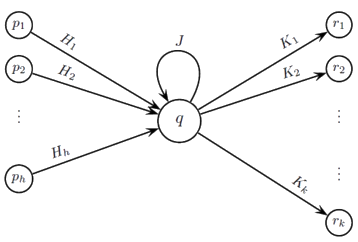
\includegraphics[width=0.5\linewidth]{automata/bmc.png}
\end{figure}

Replace $q$ with: for each pair $p_i$, $r_j$ a compensating transition $p_i \xrightarrow{H_iJ^*K_j} r_j$. All the parallel transitions should be merged ASAP in $p \xrightarrow{e_1|e_2} r$.
